\documentclass[twocolumn]{article}
\usepackage{graphicx}
\usepackage{amsmath}
\usepackage{booktabs}
\usepackage{multicol}
\usepackage{multirow}
\usepackage[margin = 2cm]{geometry}
\usepackage{array}
\usepackage{xcolor}
\usepackage[export]{adjustbox}

\begin{document}

\begin{titlepage}
    \centering
    \vspace*{-2cm}
    
\includegraphics[width=0.4\textwidth]{UoM.jpg}
    \vspace{1.5cm}

    {\LARGE University of Moratuwa}\\[0.5cm]
    {\large Department of Electronic \& Telecommunication Engineering}\\[2cm]
    
    {\Large EN1190 - Engineering Design Project}\\[0.5cm]
    {\Large Report}\\[1.5cm]
    
    \textbf{\Large Solar Wifi Router}\\[2cm]
    
    \begin{minipage}{0.4\textwidth}
        \begin{flushleft}
        \centering
            \textbf{\large Ahamed M.B.S.A. – 200014B}\\
        \end{flushleft}
    \end{minipage}
    
    \vfill
    
    {\large THIS REPORT IS SUBMITTED IN PARTIAL FULFILLMENT OF THE REQUIREMENTS FOR THE MODULE}\\[0.5cm]
    {\large EN1190 - Engineering Design Project}\\[0.5cm]
    {\large 07th of October 2023}
    
\end{titlepage}

\begin{abstract}
    We build a Wi-Fi and LED UPS system to work in power cut times or an out place that we can’t get an A/C current source. We design it in a proper way to handle it easily. We provide a 12 V rechargeable battery to charge with an A/C current (converting 230V 
    to 12V) or with a 12 V solar grid power. we use relay to perform in power cut times that     convert the power line to direct battery line. From this process, we can work with Wi- Fi and LED continuously. When we get a direct current line from any sources (A/C or solar) relay automatically convert battery line to power line. Real time we can charge the battery also is one of the benefit from this device. We can manage this process with the switches according to our required function. PCB design with the simple electronic components and enclosure is very user friendly to handle.
\end{abstract}

\section*{Introduction}
    \subsection*{1. Problem Validation}
    Due to the economic crisis in our country, there are several problems facing by students \& employees. With regard to this fuel crisis, all schools and universities are closed and the studies and works are going on the online platform. Most of students and employees are using Wi-Fi routers for access to the internet. People face many inconveniences because of sudden Wi-Fi disconnectivity caused by momentary power cuts. So, the students and workers are can’t attend the online classes, and can’t do their examinations and online submissions due to the lack of power in their devices (laptops, phones, E-tablets). And also, during the power cut hours, they can’t get proper coverage and can’t access the internet.
    
    \subsection*{2. Problem Description}
    Wi-Fi is a major service that people rely on daily to fulfil both personal and work-related duties. Currently, as the world has moved on to a norm of working from home, people rely on the home Wi-Fi connection for all their work-related needs. People face many inconveniences because of sudden Wi-Fi disconnectivity caused by momentary power cuts. Some of these inconveniences are listed below.
    
    \begin{itemize}
        \item Restarting of the router during the switch over to the generator or sudden power comebacks. 
        \item Disconnecting from important meetings or lectures. 
        \item Halting of time-critical tasks.
    \end{itemize}

    \noindent We conduct a survey on our product design, what 
    difficulties do u face when the power cut occurs, and 
    also, we mainly focused take a survey on the students 
    to identify what are the difficulties they face when 
    power cut. Because they are mainly using online 
    studies while the covid 19 pandemic situation after that 
    our country encountered fuel shortage and as a result 
    of that we have to face several hours of a power cut, so 
    we planned to make product afterward conducting 
    survey what many of them suggest and also what are 
    the alternate methods also they suggest we considered 
    them

    \noindent By considering the responses, we came up with 
    a product, which supplies power, up to 3 hours 
    during power cut. Working time will increase 
    furthermore, if solar panel output voltage is 
    sufficient. In our country we can produce the 
    power not only with fuel and coal but also there 
    are many renewable energies to produce the 
    power. So, we discussed this and came to a 
    final decision to use solar power to produce 
    electric power. Even though the majority prefer 
    to use solar energy, by considering the cost and 
    the availability of solar panels, we concerned 
    about the 2nd option, home main current too. So 
    we came up to design a product, which works 
    with main current and solar current. When the 
    output voltage of the solar panel is insufficient, 
    it will work with the main current, even though 
    if there is not a solar panel, it will work. So the 
    solar panel is optional. We decided to add a 
    darkness-sensitive LED light, which will 
    automatically on during power cut and in 
    darkness.

\section*{Components}
We use basic electronic components to build the PCB to work with this system

\subsection*{1. LM317T Regulator:}
15V – 0 – 15V Transformer
15-0-15 1A Centre Tapped Step Down 
Transformer is a general purpose chassis 
mounting mains transformer. Transformer has 
230V primary winding and centre tapped 
secondary winding. The transformer has flying 
colored insulated connecting leads (Approx.
100 mm long). The Transformer act as step 
down transformer reducing AC - 230V to AC -
15V.

\noindent The Transformer gives outputs of 15V, 15V and 
0V. The Transformer's construction is written 
below with details of Solid Core and Winding.

\begin{figure}[h]
    \centering
    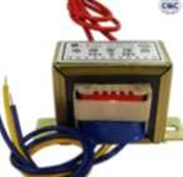
\includegraphics{1.png}
    \label{fig:enter-label}
\end{figure}

\noindent The transformer is a static electrical device that 
transfers energy by inductive coupling between 
its winding circuits. A varying current in the 
primary winding creates a varying magnetic 
flux in the transformer's core and thus a varying 
magnetic flux through the secondary winding. 
This varying magnetic flux induces a varying 
electromotive force (E.M.F) or voltage in the 
secondary winding. The transformer has cores 
made of high 
permeability silicon 
steel. The steel has a 
permeability many 
times that of free 
space and the core 
thus serves to greatly 
reduce the 
magnetizing current and confine the flux to a 
path which closely couples the winding.
\vspace{5pt}

\noindent Specifications of 15-0-15 1A Centre Tapped Transformer: - 

\noindent Input Voltage: 230V AC \\
Output Voltage: 15V, 15V or 0V \\
Output Current: 1Amp \\ 
Mounting : Vertical mount type \\

\subsection*{2. Regulator (24V – 14.8V)}
24V to 14.8V Converter using LM317T IC, 7812 , 7824 
\vspace{1pt}

\noindent 24V-to-14.8V-Converter-using-LM317T-ICPower-Supply
\vspace{5pt}

\noindent So ever wondered how come some circuit takes 
a 24V input but is internally driving LED’s 
Microcontrollers and other low voltage 
peripherals which are not even designed for 
such a high voltage? For a newbie, the first 
thought might be 
making a voltage 
divider circuit and thus 
supplying the desired 
voltage as such, but this 
is not how it’s done.
\vspace{1pt}

\begin{figure}[h]
    \centering
    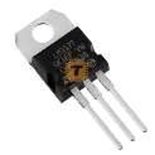
\includegraphics{2.png}
    \label{fig:enter-label}
\end{figure}

\noindent The losses in a voltage divider circuit and the 
uncertainty of a load that does not have a fixed 
resistance makes this hardly the best possible 
way to tackle it. So that is where a regulator IC 
comes in such as the infamous 317T.

\noindent The 317T is used a lot in circuits with a 
minimum footprint required to convert their 
voltage from a higher level to 5V. The 
component list is very small and is great for 
hobby and semi-professional to professionalgrade projects in general. So let’s get started!


\subsection*{2. Zener diode (6.8V) ):}

Features: \\

\noindent Standard 6.8V Zener Diode \\
Nominal Zener Voltage (Vz): 6.8V \\
Maximum Regulator Current (Izm): 0.055A \\
Max. Reverse Leakage Current (Ir): 0.1µA \\
Forward Voltage Drop (Vf): 1.5V \\
Total Power Dissipation (P tot): 500mW \\
\vspace{5pt}

\noindent Description: \\

\noindent The 1N754 Zener Diode is 
a standard 6.8V Zener 
Diode with a low leakage 
current and accurate 
working voltage. The 1N754 is ideal for use in 
clamping applications and protection circuits.


\subsection*{3. Rectifier Module (1A)}
In the electronics industry, one of the most 
popular applications of semiconductor diodes is 
to convert alternating current (AC) signal of 
any frequency, which is typically 60 or 50 Hz, 
to a direct current (DC) signal. This DC signal 
can be used for powering electronic devices, 
rather than batteries. The circuit which converts 
the AC into DC signal commonly consists of a 
particular arrangement of 
interlocked diodes and is 
known as a rectifier. In 
power supply circuits, 
two types of rectifier 
circuits are commonly 
used — half-wave and 
full-wave. Half-wave 
rectifiers only permit 
one-half of the cycle through, whereas fullwave rectifiers permit both the top half and 
bottom half of the cycle through, while 
converting the bottom half to the same polarity 
as the top.

\begin{figure}[h]
    \centering
    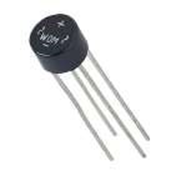
\includegraphics{3.png}
    \label{fig:enter-label}
\end{figure}

\noindent Between the two types, the full-wave rectifier is 
more efficient as it uses the full cycle of the incoming waveform. There are two types of 
full-wave rectifiers — the centre-tapped fullwave rectifier, which requires a centre-tapped transformer, and the bridge rectifier, which does 
not need a centre-tapped transformer.

\subsection*{4. Relay Module (24V, 12V)}
A relay is an electrically operated switch. It 
consists of a set of input terminals for a single 
or multiple control signals, and a set of 
operating contact terminals. The switch may 
have any number of contacts in multiple contact 
forms, such as make contacts, break contacts, or 
combinations thereof.
Relays are used where it is necessary to control 
a circuit by an independent low-power signal, 
or where several circuits must be controlled by 
one signal. Relays were first used in long-distance 
telegraph circuits as signal repeaters: they 
refresh the signal coming in from one circuit by 
transmitting it on another circuit. Relays were 
used extensively in telephone exchanges and 
early computers to perform logical operations.

\noindent The traditional form of a relay uses an 
electromagnet to close or open the contacts, but 
relays using other operating principles have also 
been invented, such as in solid-state relays 
which use semiconductor properties for control 
without relying on moving parts. Relays with 
calibrated operating characteristics and 
sometimes multiple operating coils are used to 
protect electrical circuits from overload or 
faults; in modern 
electric power 
systems these 
functions are 
performed by digital 
instruments still 
called protective 
relays.

\begin{figure}[h]
    \centering
    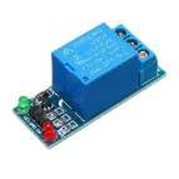
\includegraphics{4.png}
    \label{fig:enter-label}
\end{figure}

\noindent Latching relays require only a single pulse of 
control power to operate the switch persistently. 
Another pulse applied to a second set of control 
terminals, or a pulse with opposite polarity, 
resets the switch, while repeated pulses of the 
same kind have no effects. Magnetic latching 
relays are useful in applications when 
interrupted power should not affect the circuits 
that the relay is controlling.


\subsection*{5. Purpose of switch}
Switches are used for manually control LED and Wi-Fi router. You can use this device in power off times manually.  

\begin{figure}[h]
    \centering
    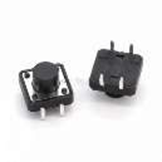
\includegraphics{5.png}
    \label{fig:enter-label}
\end{figure}


\subsection*{6. Other Components}

listed the other components we have used except the components listed above

\begin{table}[htbp]
    \centering
    \caption{Components and Values}
    \begin{tabular}{lll}
        \toprule
        \textbf{Component} & \textbf{Value} & \textbf{Quantity} \\
        \midrule
        3 core wires & 16/0.20 mm & 2m \\
        Plug top & & 1 \\
        IC & 7824 & 1 \\
        & 7812 & 1 \\
        Switch & & 2 \\
        LED strip & & 1 \\
        Resistor & 2.2 K$\Omega$ & 2 \\
        & 1 K$\Omega$ & 2 \\
        & 240 $\Omega$ & 1 \\
        & 100 $\Omega$ & 1 \\
        Preset resistor & 1 K$\Omega$ & 1 \\
        & 200 K$\Omega$ & 1 \\
        IN 4007 diode & & 5 \\
        Li-ion Battery & 3.7V & 4 \\
        Capacitor & 2.2mF & 1 \\
        & 0.33$\mu$F & 3 \\
        & 0.11$\mu$F & 3 \\
        Transistors & C828 & 1 \\
        & D400 & 1 \\
        & BD 139 & 1 \\
        LED & Red & 1 \\
        & Green & 1 \\
        \bottomrule
    \end{tabular}
\end{table}

\section*{Method}
\section*{1. How to Work with the Device}
\begin{enumerate}
    \item Keep the device on your table or hang it on the wall properly.
    \item Connect the 230V A/C adapter to the pin labeled "A/C power in."
    \item Connect the Wi-Fi router cable to the Wi-Fi pin.
    \item (Optional) Connect the Solar Panel cable to the solar panel pin (if available).
\end{enumerate}

\subsection*{2. Configuring the device}
Connect your devices (LED, Wi-Fi) and power 
on your A/C power in, while working, your 
battery will charge with the use of solar energy 
and in the case of output voltage is not 
sufficient it will automatically charge from 
main current. So, solar panel is optional and 
user can use this product without solar panel.
When charging, the green LED will on and, red 
LED will indicate battery is fully charged.
The Wi-Fi and 12V LED is now working on 
using A/C power in.

\section*{PCB Design}
The schematic of the circuit was drawn first, and the PCB was designed accordingly using Altium. To optimize space, the PCB was made as small as possible. Lines were routed on both the top and bottom layers. For power lines, a thickness of 2mm was used for 24V, and 1.5mm for 12V. Other lines were routed around 0.75mm.

\section*{Finalized Sketch of the Enclosure (3D)}
Initially, an enclosure was designed to physically connect the components, ensuring that the circuit worked as intended. Afterward, the focus shifted towards creating a user-friendly interface. The final enclosure design was made to be straightforward, resembling normal electronic devices. A significant effort was put into providing an easy-to-use interface so that anyone can handle the device effectively.

\section*{PRODUCT ARCHITECTURE}

\begin{figure}[h]
    \centering
    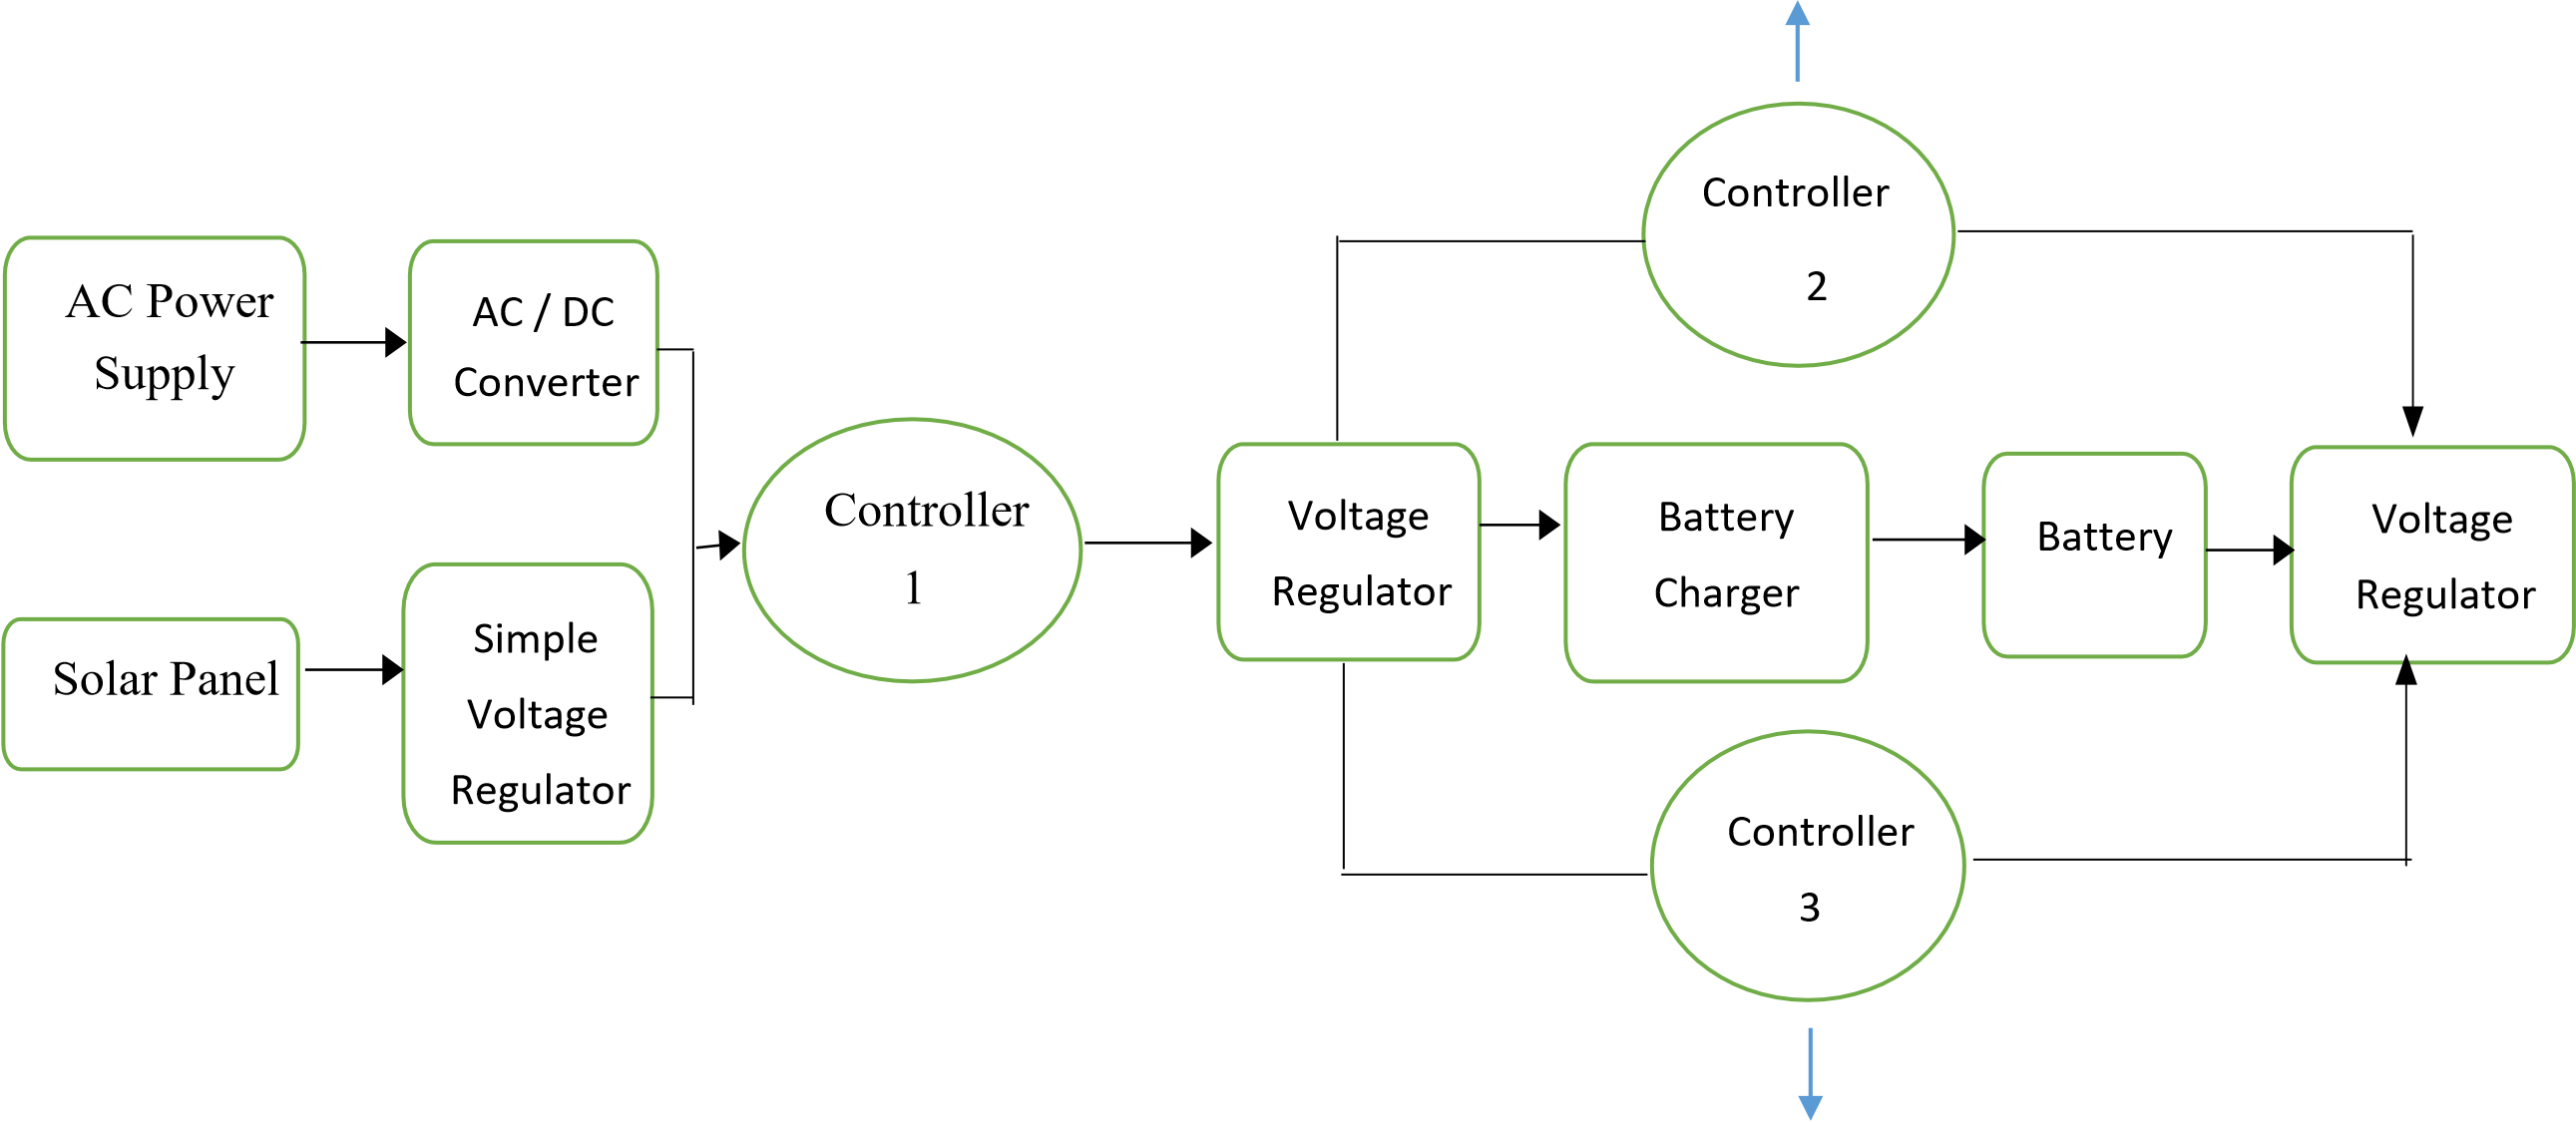
\includegraphics[width = 8cm]{6.png}
    \label{fig:enter-label}
\end{figure}

\section*{Technical Aspects}
\subsection*{1. Controller 1}
During optimal sunshine, the relay gets sufficient power from the panel and remains switched ON with its N/O contacts activated. If the solar panel's output voltage is insufficient, RL2 relay will automatically give power to the circuit using the main current. So this product will work without a solar panel too.

\subsection*{2. Voltage Regulator}
Since the output of the solar panel is unregulated DC voltage, LM317T IC (U1) is used to provide regulated DC voltage. \\

\noindent LM317T \\


\noindent The LM317T is a positive adjustable voltage regulator designed to supply more than 1.5 A of load current with an output voltage adjustable over a 1.2 to 37 V range. The nominal output voltage is selected by means of only a resistive divider. 

\begin{figure}[h]
    \centering
    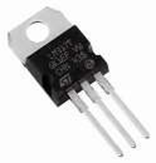
\includegraphics{7.png}
    \label{fig:enter-label}
\end{figure}

\noindent For this circuit, the input voltage of the LM317T is about 18V, and the output voltage is adjusted to 14.8V (since we are using a 14.8V battery). A potentiometer (10k) is used to adjust the output voltage of this voltage regulator LM317.

\subsection*{3. Battery Charger}

\begin{figure}[h]
    \centering
    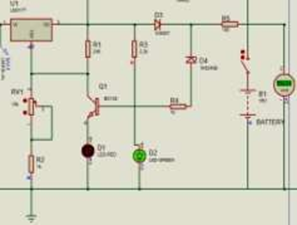
\includegraphics{8.png}
    \label{fig:enter-label}
\end{figure}

\begin{figure}[h]
    \centering
    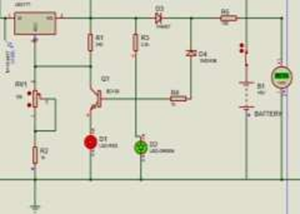
\includegraphics{9.png}
    \label{fig:enter-label}
\end{figure}

\noindent When the battery voltage is below 14.8V, current from LM317 IC flows through the resistor R5 and diode D3 to the battery, and the Zener diode will not conduct. 
\vspace{1pt}

\noindent Green LED is indicating the charge of the battery. Resistor R3 is used to protect the green LED from high voltages. 
\vspace{1pt}

\noindent When the battery voltage rises to 16V, the current flow to the battery stops, and the Zener diode gets sufficient breakdown voltage, allowing the current through it. 
\vspace{1pt}

\noindent Now the base of the transistor gets sufficient current to turn on, and the Red LED will turn on. The Red LED indicates that the battery is fully charged. 
\vspace{1pt}

\noindent Diode D3 is used to avoid the discharge of the battery when the output from the solar panel is very low.

\subsection*{4. Battery Voltage Regulator}
Since the output voltage of the battery is unregulated, the 7812 voltage regulator is used to get a steady 12V voltage. 

\begin{figure}[h]
    \centering
    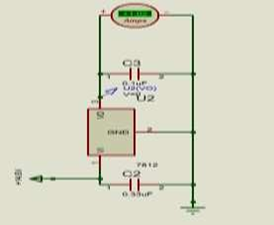
\includegraphics{10.png}
    \label{fig:enter-label}
\end{figure}

\subsection*{7812 voltage regulator}
The 7812 is a fixed voltage linear regulator that can output 12V at up to 1A current with an input voltage range of 14–35V. 

\begin{figure}[h]
    \centering
    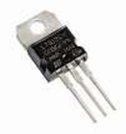
\includegraphics{11.png}
    \label{fig:enter-label}
\end{figure}

\noindent R8 is used to reduce the current from 1A to 0.5A.

\subsection*{5. Controller 2}
When sufficient solar voltage or main current is available, Wi-Fi and LED (LED is controlled by RL1) are activated; otherwise, it will automatically connect to the battery. This operation is controlled by RL3 relay. Since the output voltage of LM317T is 14.8V, the 4.7 Ohm resistor R9 is used to drop the voltage from 14.8V to 12V.

\begin{figure}[h]
    \centering
    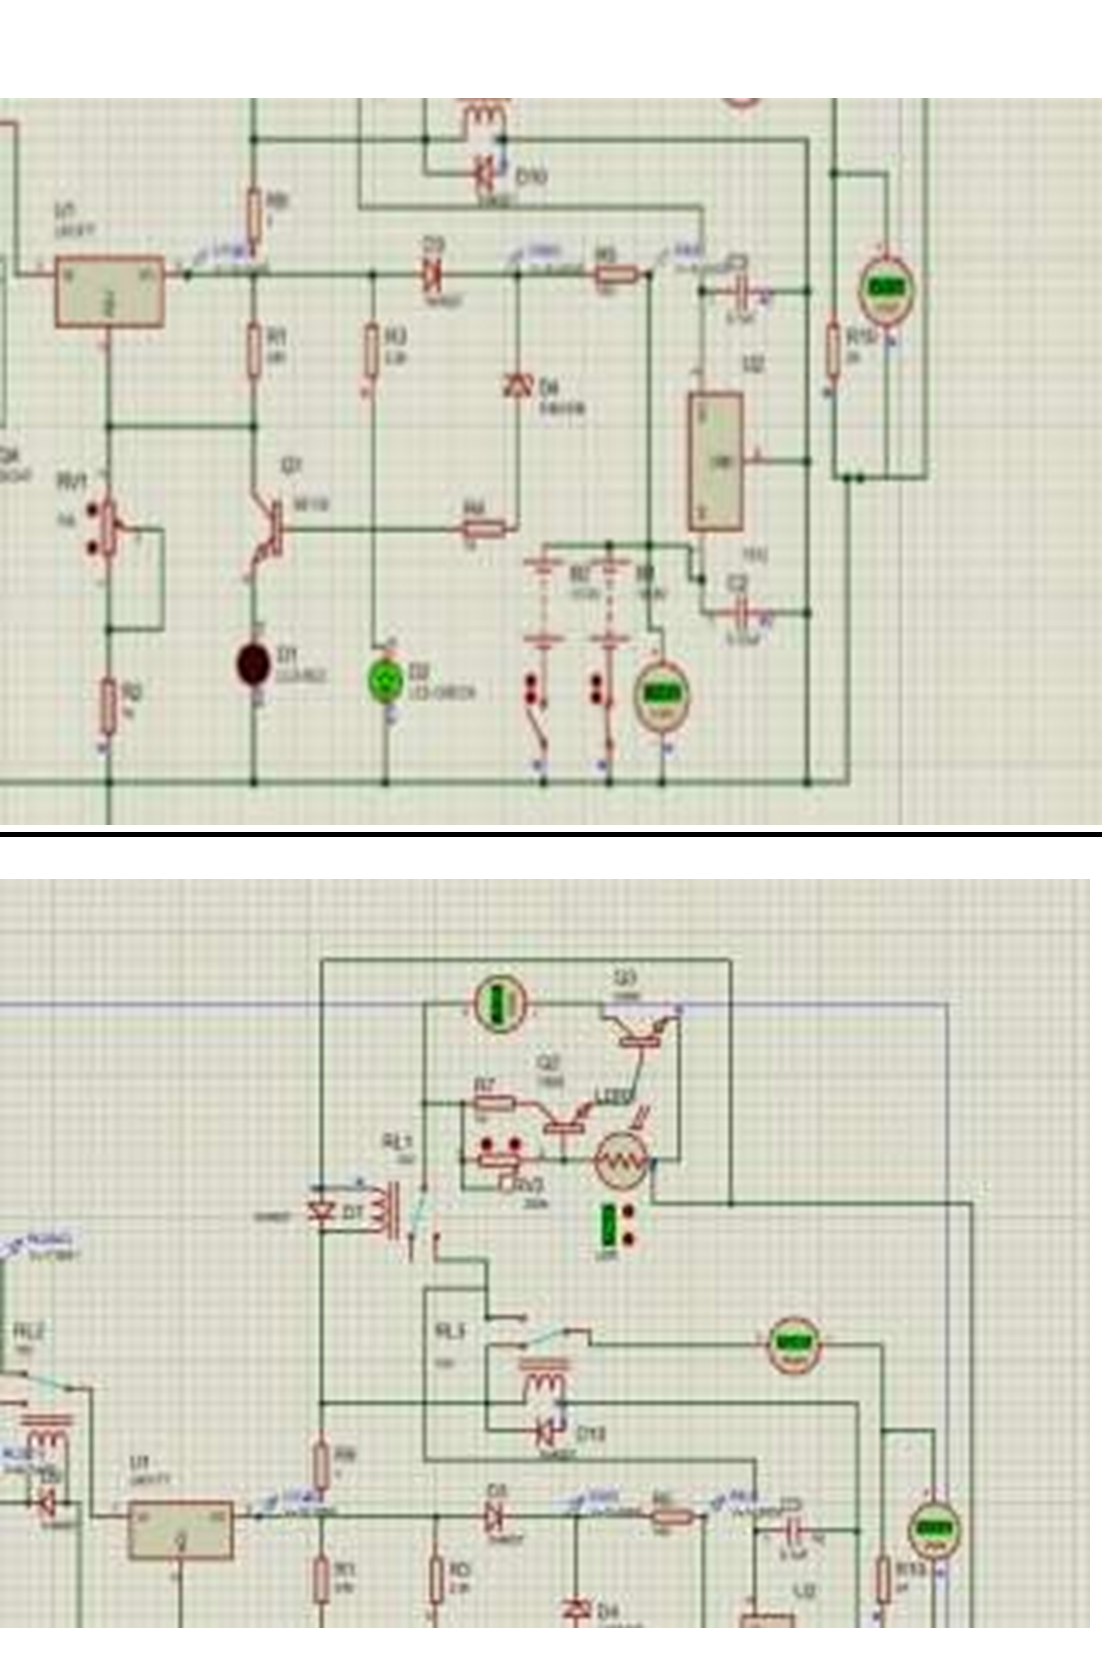
\includegraphics{12.png}
    \label{fig:enter-label}
\end{figure}

\begin{figure}[h]
    \centering
    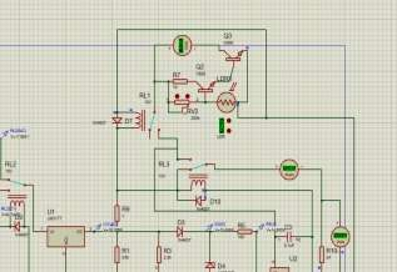
\includegraphics{13.png}
    \label{fig:enter-label}
\end{figure}

\subsection*{6. Darkness Sensitive Circuit}

\begin{figure}[h]
    \centering
    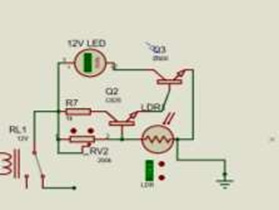
\includegraphics{14.png}
    \label{fig:enter-label}
\end{figure}

This circuit is used to automatically turn on the LED during power cut times (controlled by RL1) and in darkness (controlled by LDR). As mentioned above, the A-B point will get 12V voltage only in power cut times, and LDR resistance is very high in the darkness, causing the LED to turn on. By using the RV2 variable resistor, the operating darkness can be adjusted.

\section*{Technical Specifications}
\begin{enumerate}
    \item Key Features of Our Product:
    \begin{itemize}
        \item Real-time working
        \item Efficient power providing and easy to handle
        \item Can be used automatically and manually
    \end{itemize}
    \item Weight: 300g
    \item Physical Dimensions:
    \begin{itemize}
        \item Height: 120mm
        \item Width: 90mm
        \item Length: 180mm
    \end{itemize}
    \item Working Time: 3 hours
    \item Charging Time: 1 hour
    \item Power Consumption: 6W
    \item Warranty: 1 year
    \item Life Time: 4-5 years
\end{enumerate}


\begin{titlepage}
    \section*{Appendix}

    \subsection*{Circuit Design}
    
        \begin{figure}[h]
            \centering
            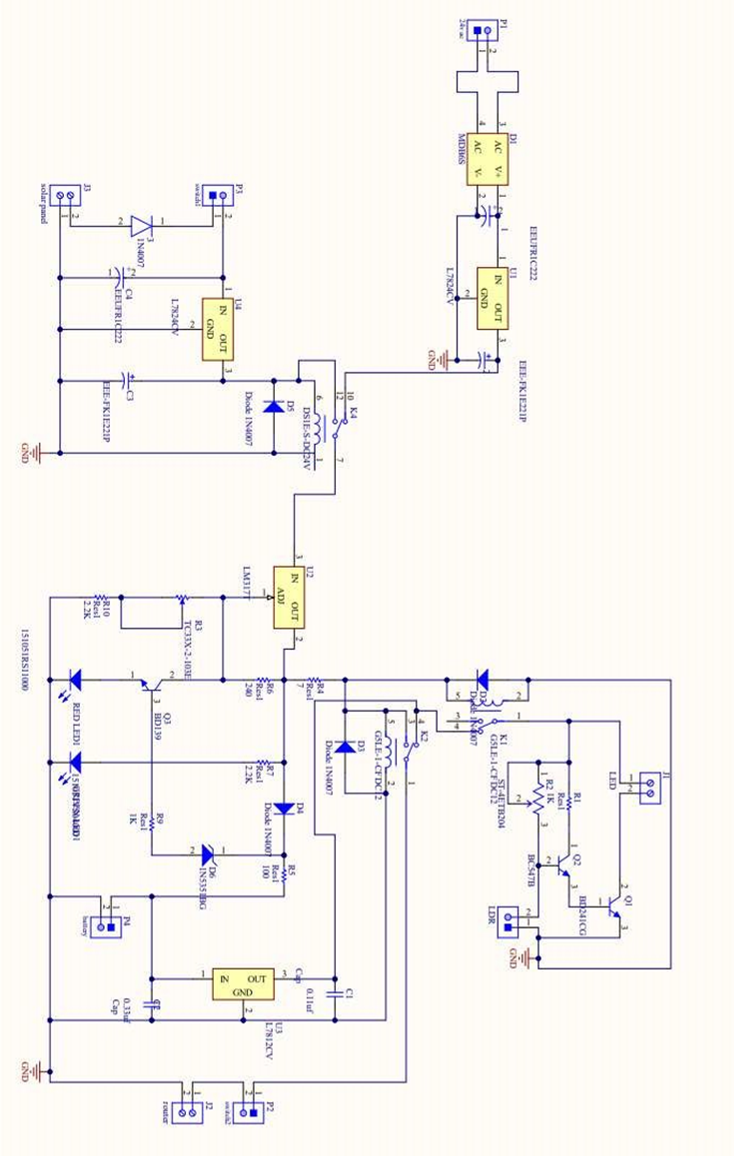
\includegraphics[width = 11.9cm]{15.png}
            \label{fig:enter-label}
        \end{figure}

    \newpage
    
    \subsection*{Proteus Simulation}

        \begin{figure}[h]
            \centering
            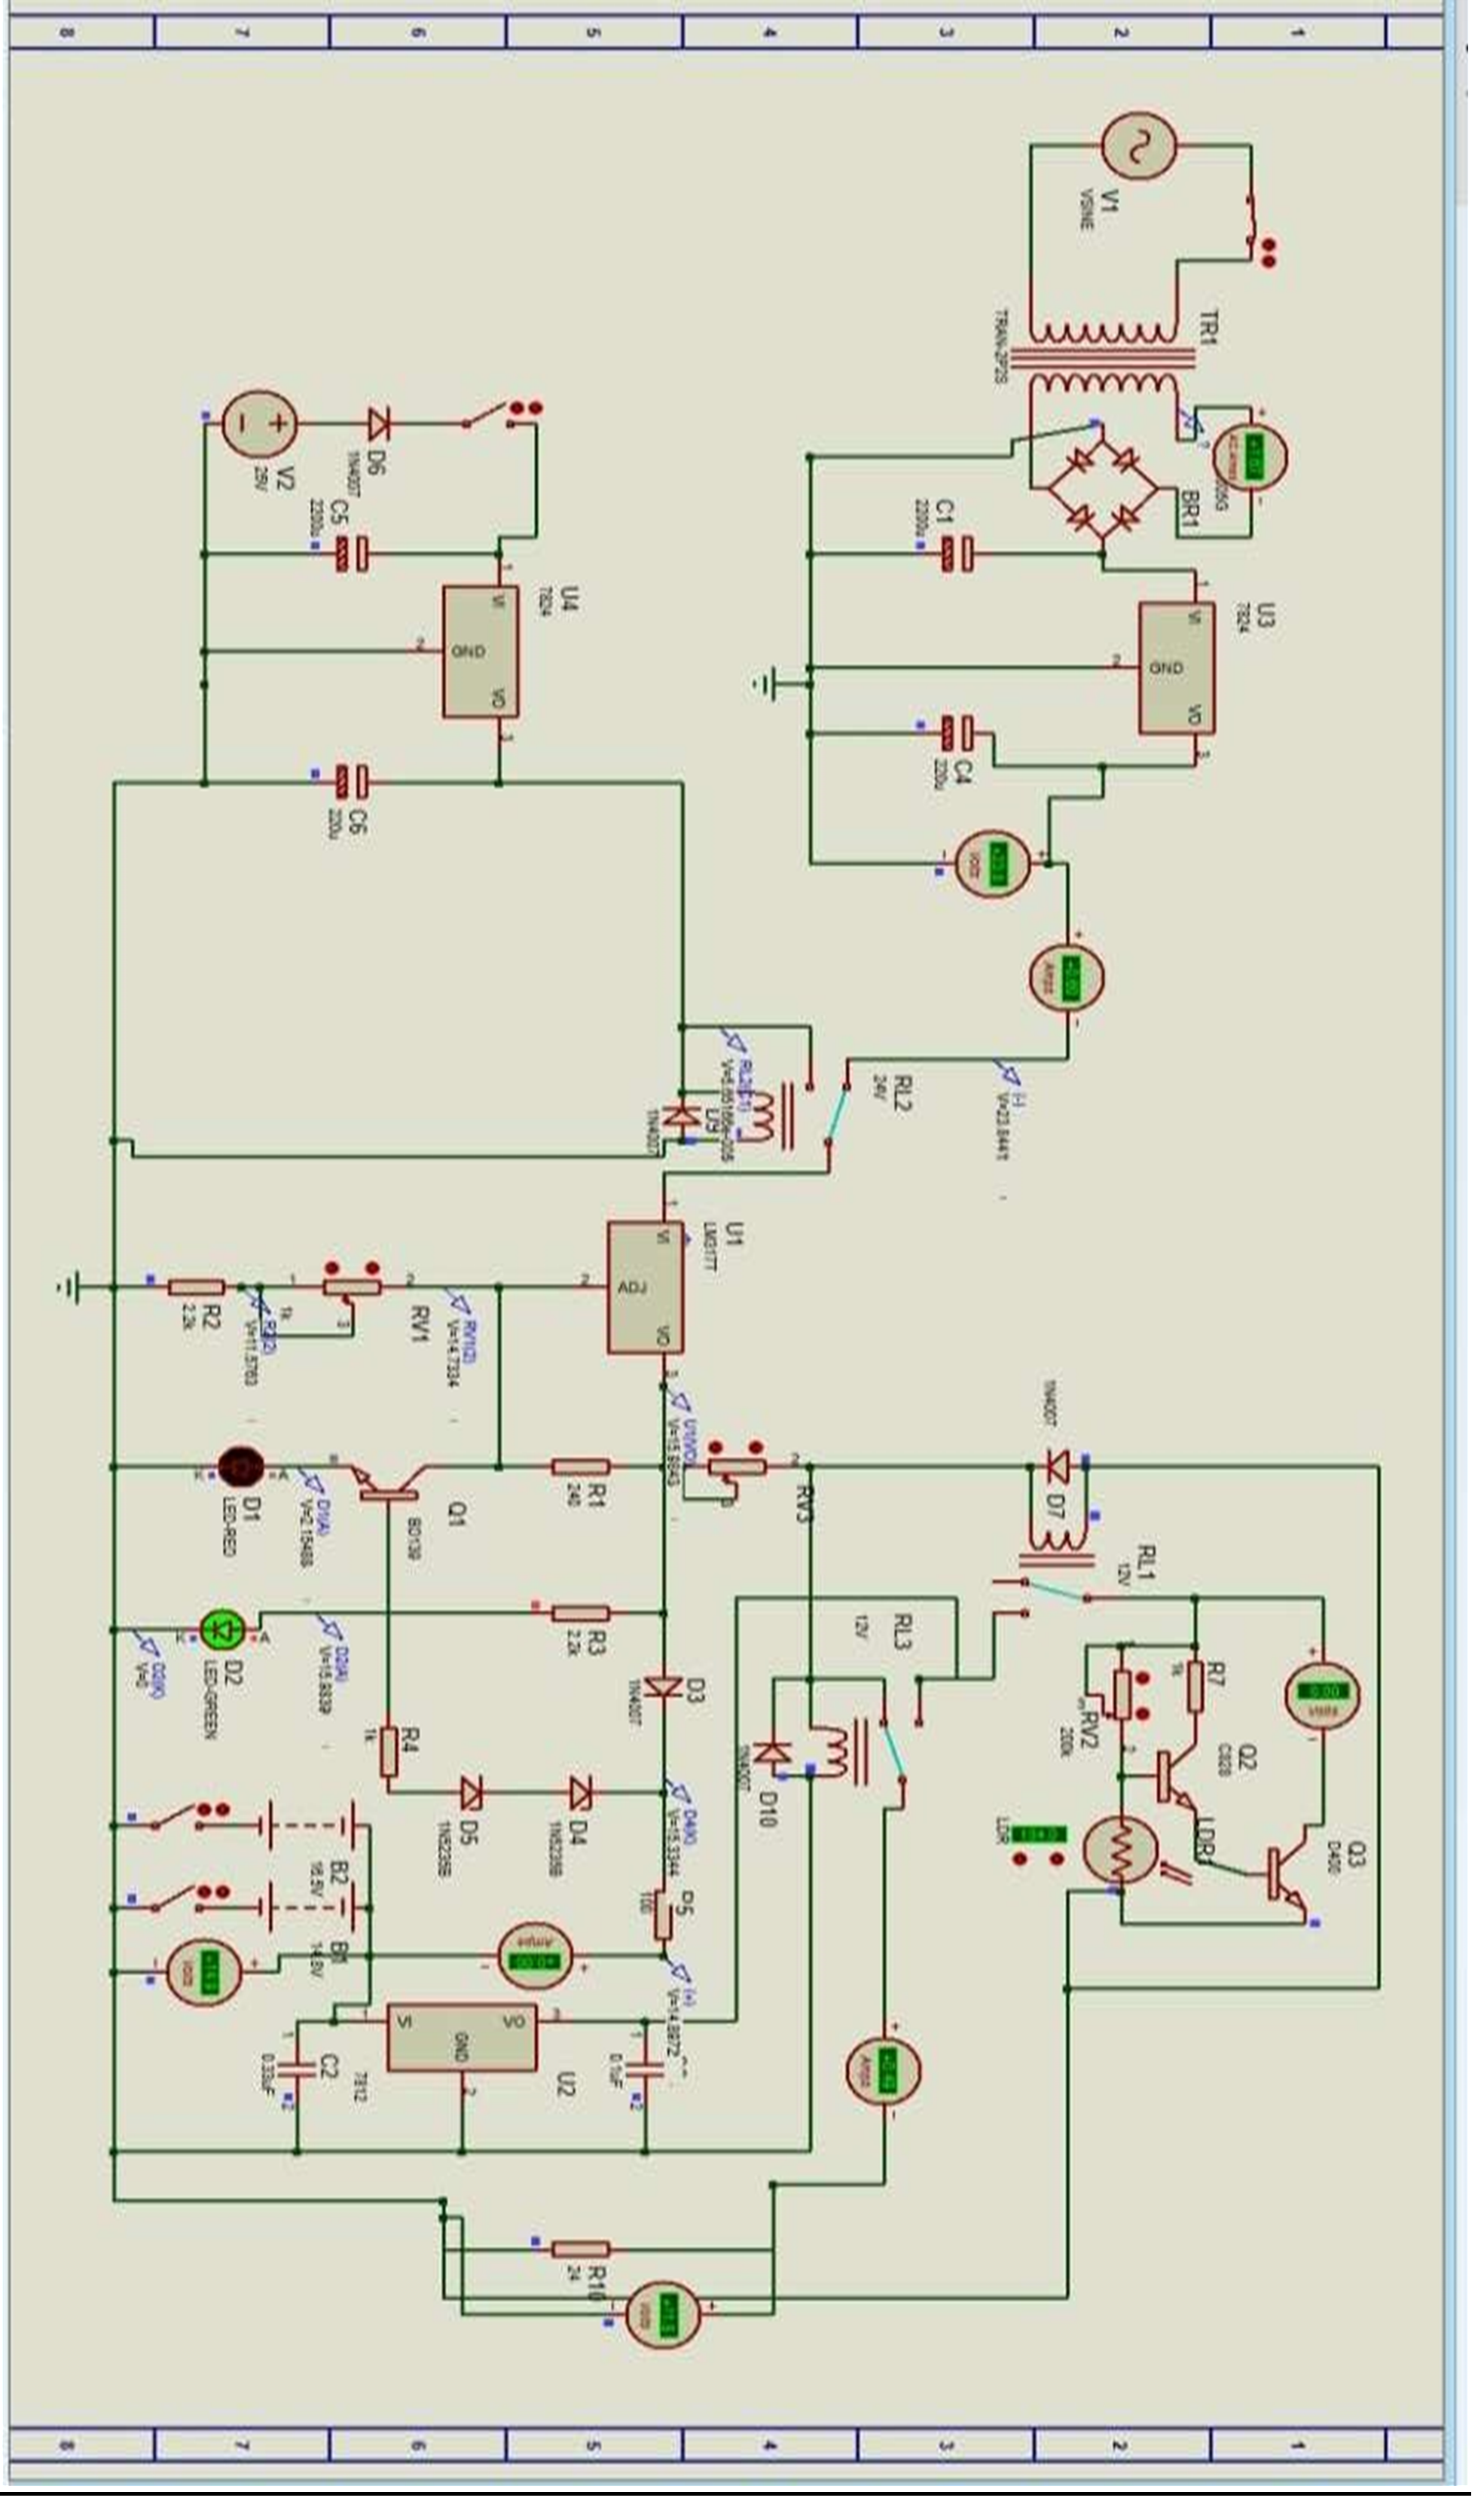
\includegraphics[width = 11cm]{16.png}
            \label{fig:enter-label}
        \end{figure}

    \newpage
    
    \subsection*{3D Enclosure}

    \begin{figure}[h]
        \begin{minipage}{0.6\textwidth}
            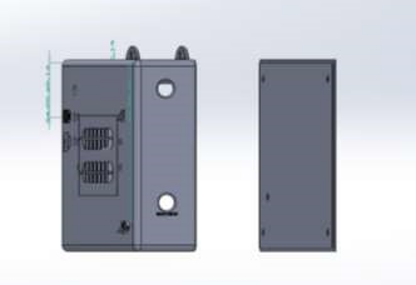
\includegraphics[width=8cm]{17.png}
        \end{minipage}
        \hfill
        \begin{minipage}{0.35\textwidth}
            \caption{Side View}
            \label{fig:enter-label}
        \end{minipage}
    \end{figure}

    \begin{figure}[h]
        \begin{minipage}{0.6\textwidth}
            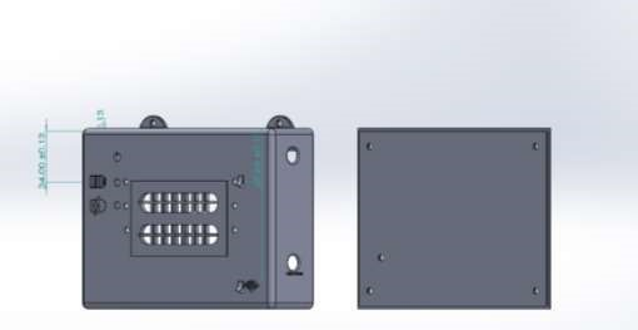
\includegraphics[width=8cm]{18.png}
        \end{minipage}
        \hfill
        \begin{minipage}{0.35\textwidth}
            \caption{Front View}
            \label{fig:enter-label}
        \end{minipage}
        
    \end{figure}

    \begin{figure}[h]
        \begin{minipage}{0.6\textwidth}
            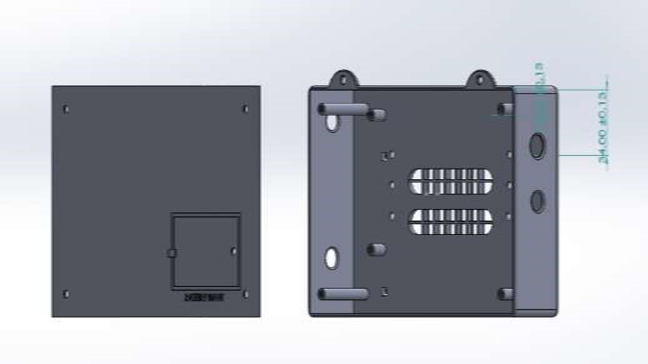
\includegraphics[width=8cm]{19.png}
        \end{minipage}
        \hfill
        \begin{minipage}{0.35\textwidth}
            \caption{Back View}
            \label{fig:enter-label}
        \end{minipage}
        
    \end{figure}    

    \begin{figure}[h]
        \begin{minipage}{0.6\textwidth}
            
\includegraphics[width=8cm]{20.png}
        \end{minipage}
        \hfill
        \begin{minipage}{0.35\textwidth}
            \caption{Up View}
            \label{fig:enter-label}
        \end{minipage}
        
    \end{figure}  

    \begin{figure}[h]
        \centering
        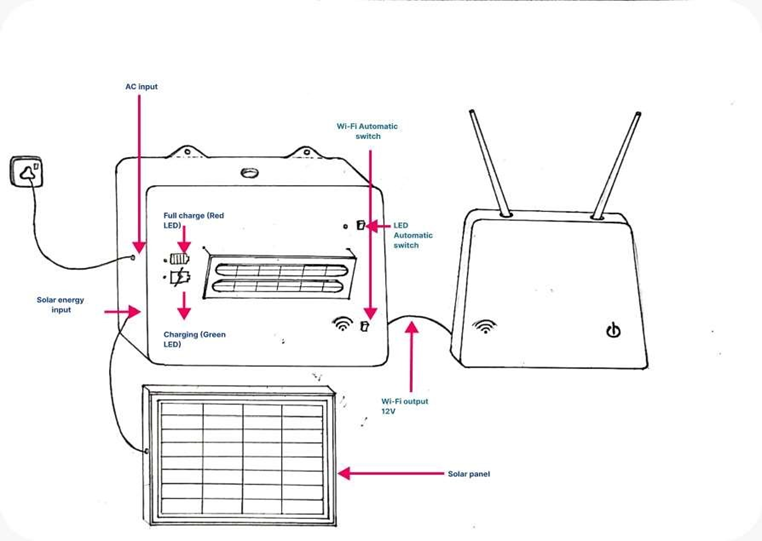
\includegraphics{21.png}
        \label{fig:enter-label}
    \end{figure}

    \begin{figure}[h]
        \centering
        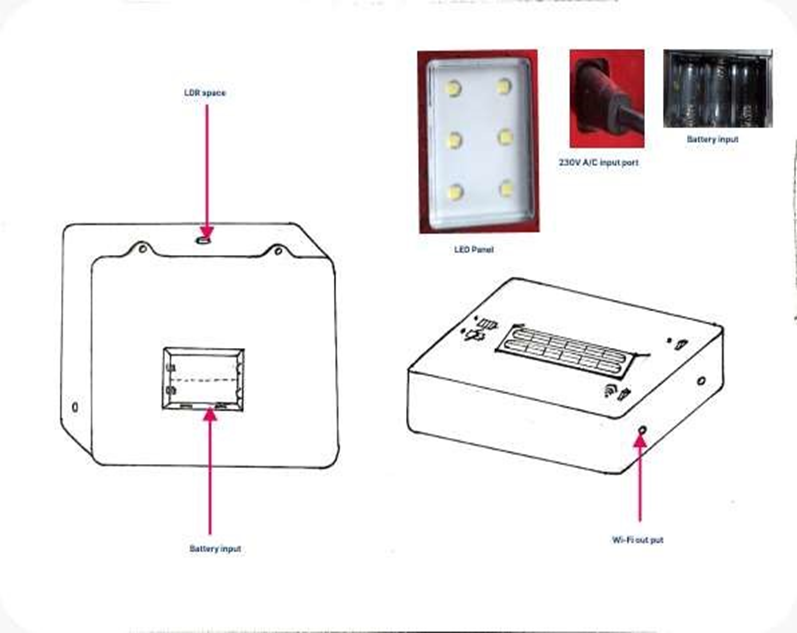
\includegraphics{22.png}
        \label{fig:enter-label}
    \end{figure}

    \newpage
\end{titlepage}

\begin{titlepage}
    \subsection*{PCB Layout (Altium Design)}
    
    \begin{figure}[h]
        \centering
        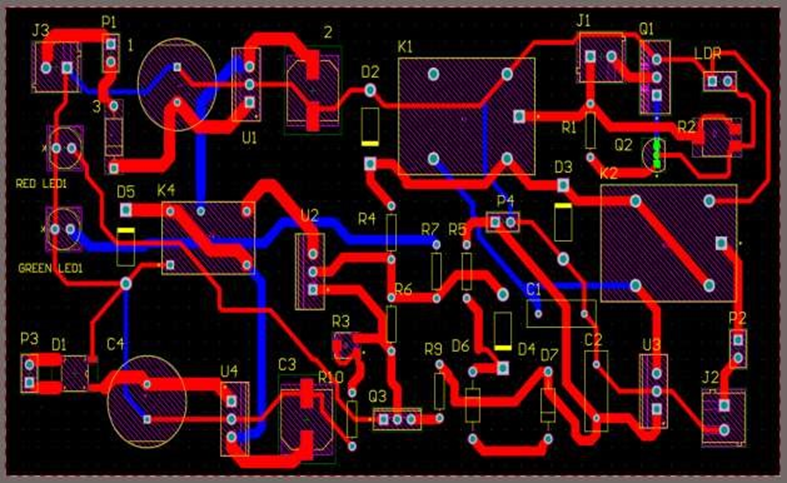
\includegraphics[width=12cm]{23.png}
        \caption{Top Layer}
        \label{fig:enter-label}
    \end{figure}

    \begin{figure}[h]
        \centering
        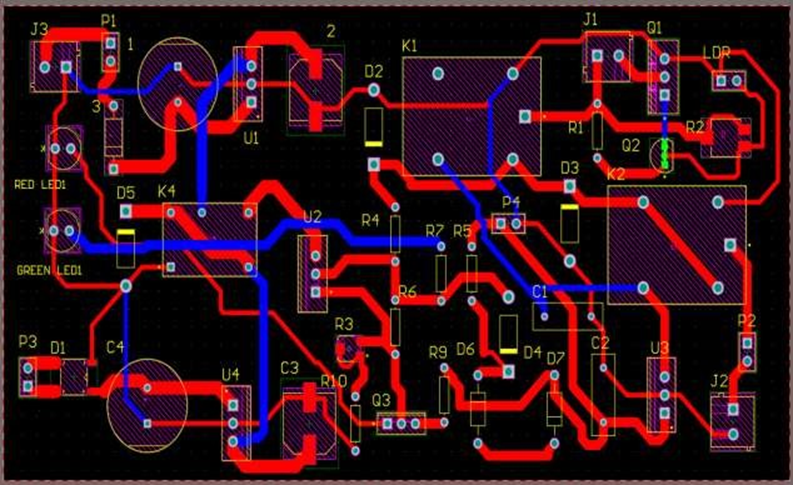
\includegraphics[width=12cm]{24.png}
        \caption{Bottom Layer}
        \label{fig:enter-label}
    \end{figure}

    \begin{figure}[h]
        \centering
        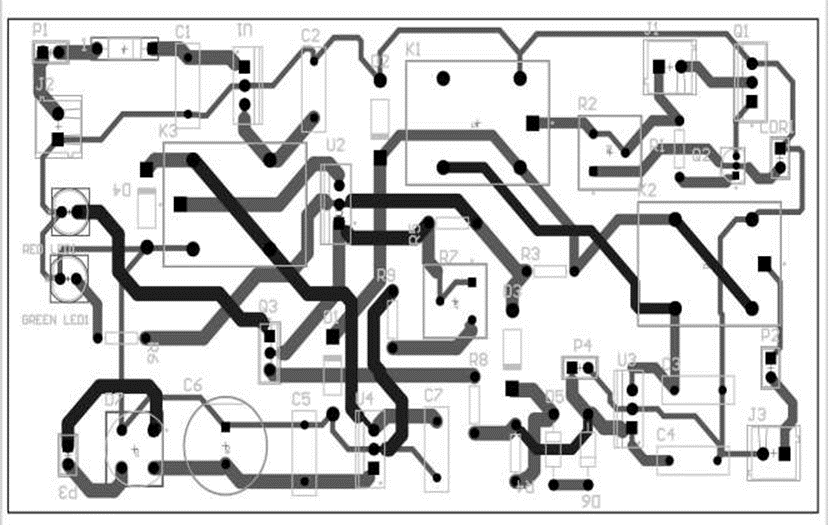
\includegraphics[width=12cm]{25.png}
        \label{fig:enter-label}
    \end{figure}

    \vspace{200pt}

    \section*{Survey Results}

    \begin{figure}[h]
        \centering
        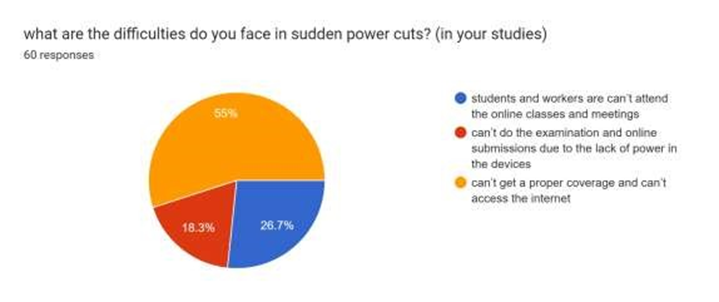
\includegraphics{26.png}
        \label{fig:enter-label}
    \end{figure}
    
    \begin{figure}[h]
        \centering
        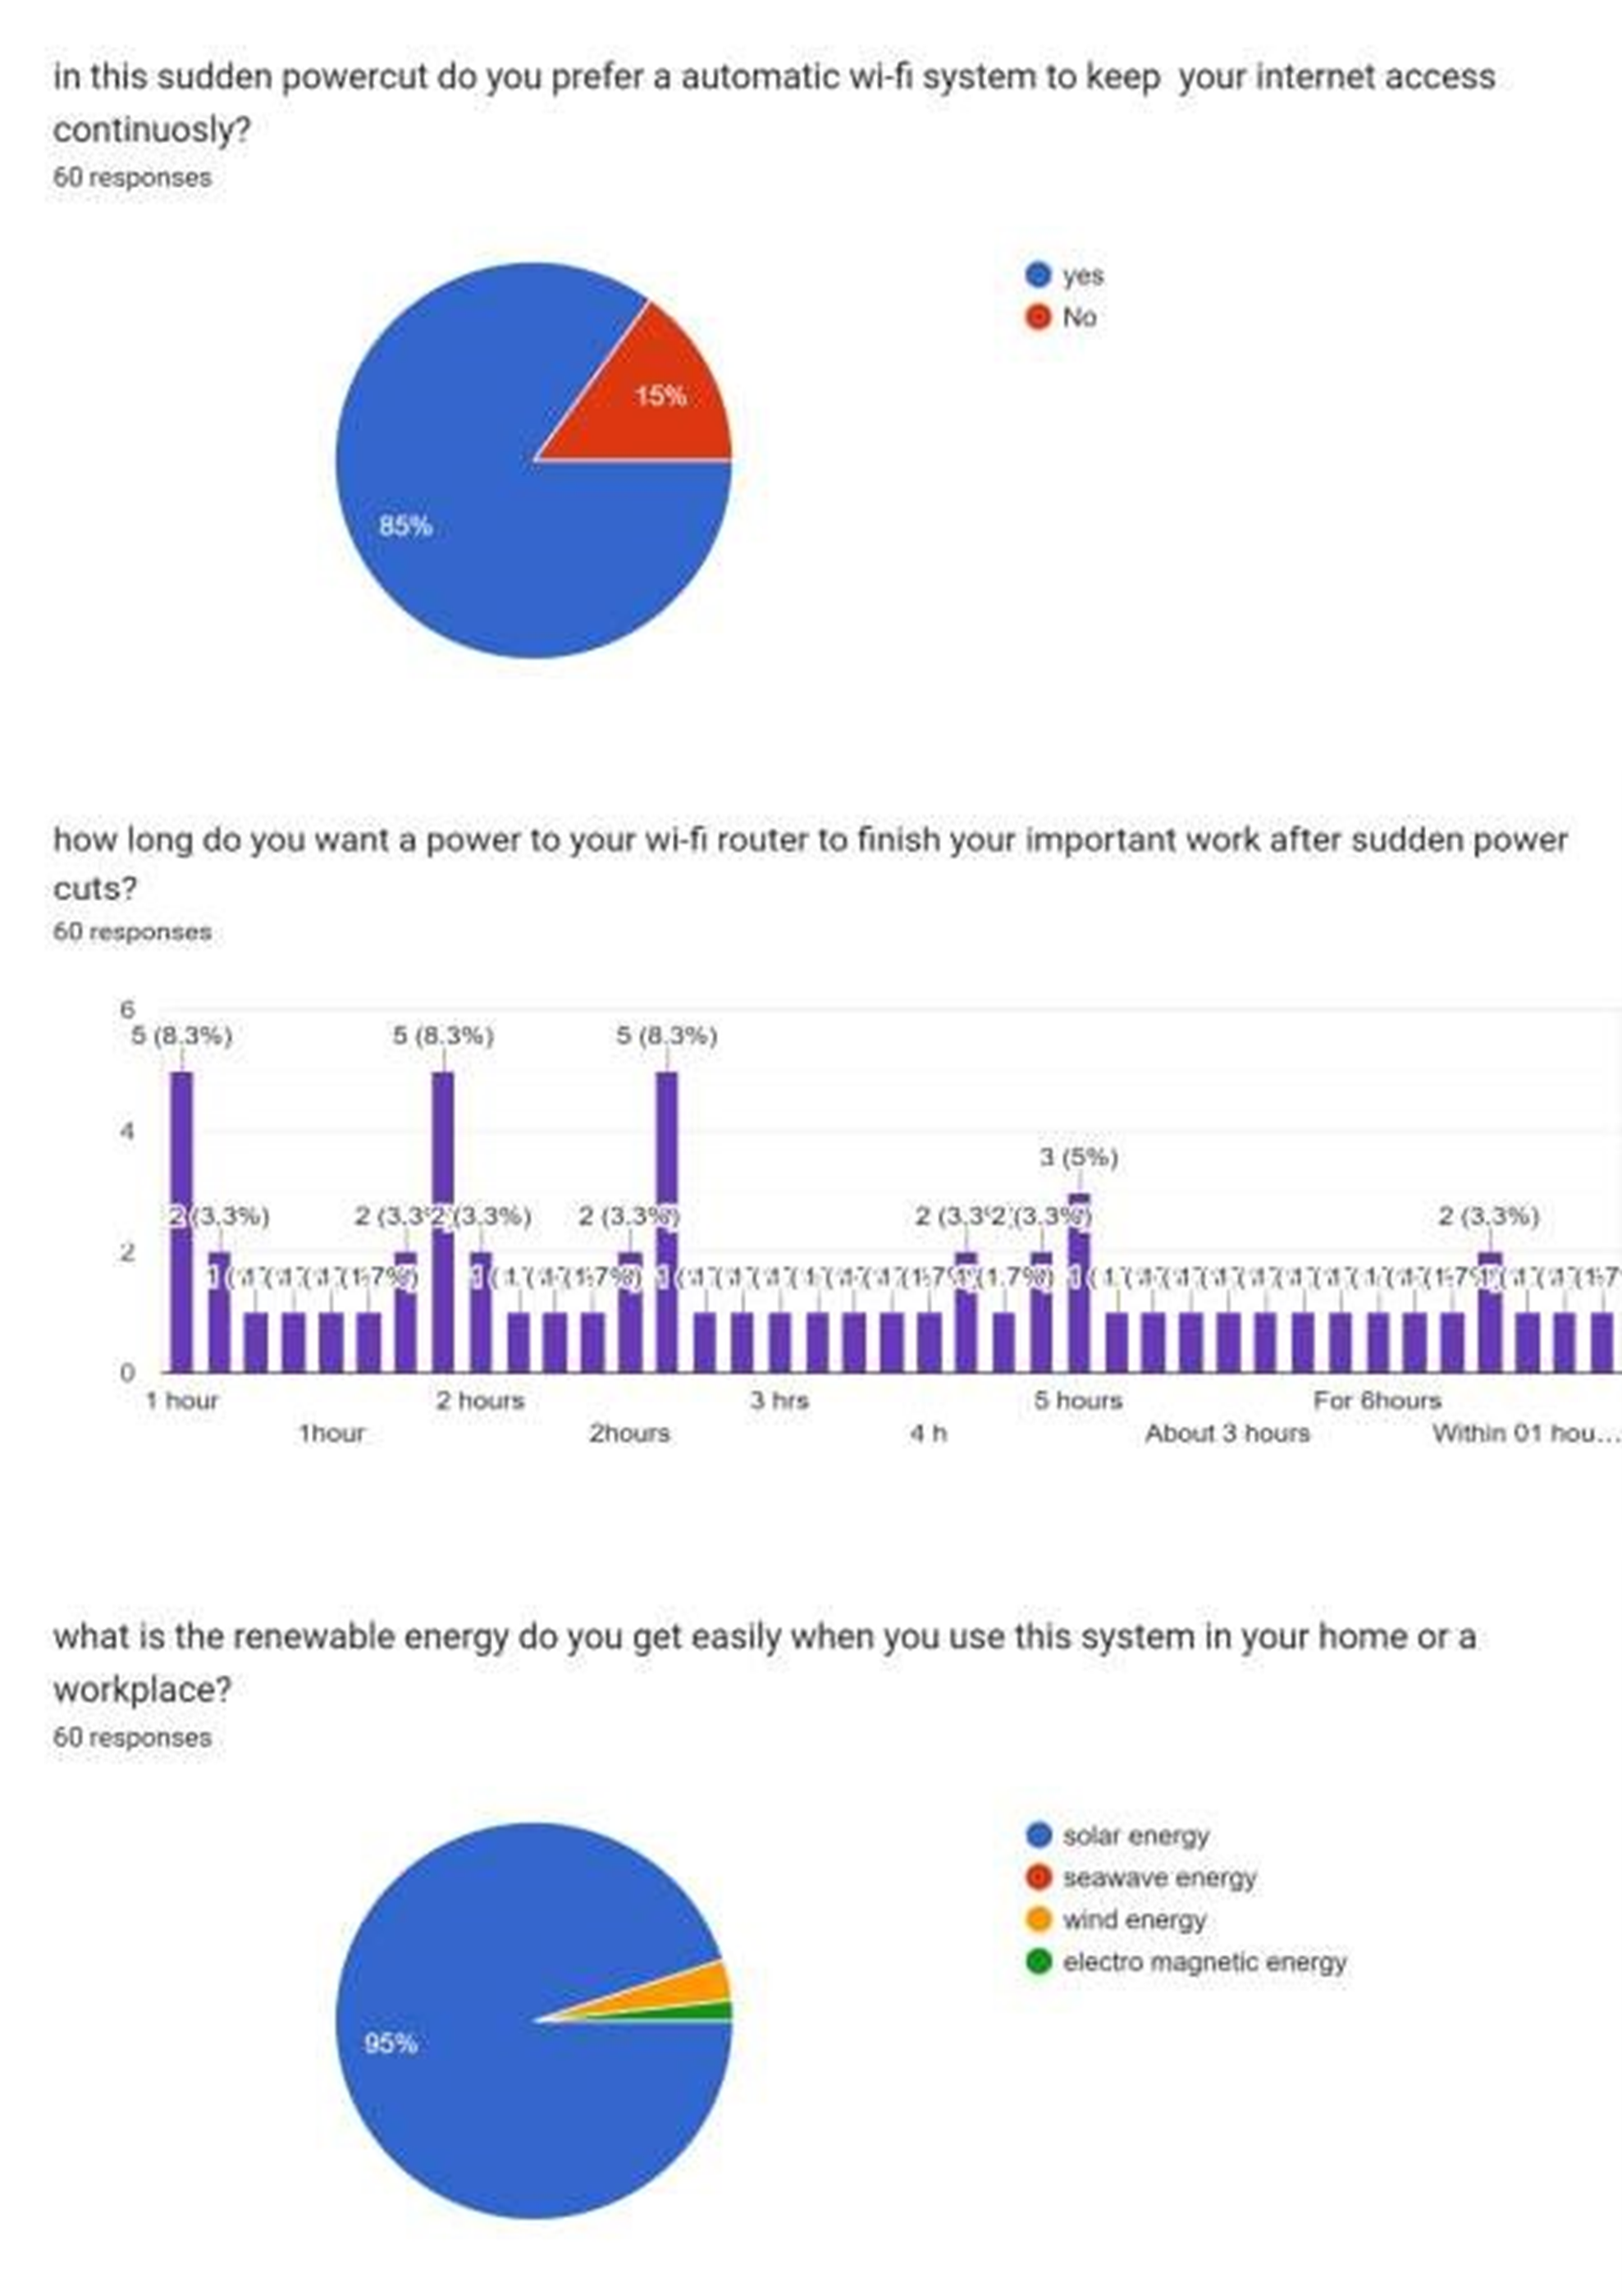
\includegraphics{27.png}
        \label{fig:enter-label}
    \end{figure}
    
    \begin{figure}[h]
        \centering
        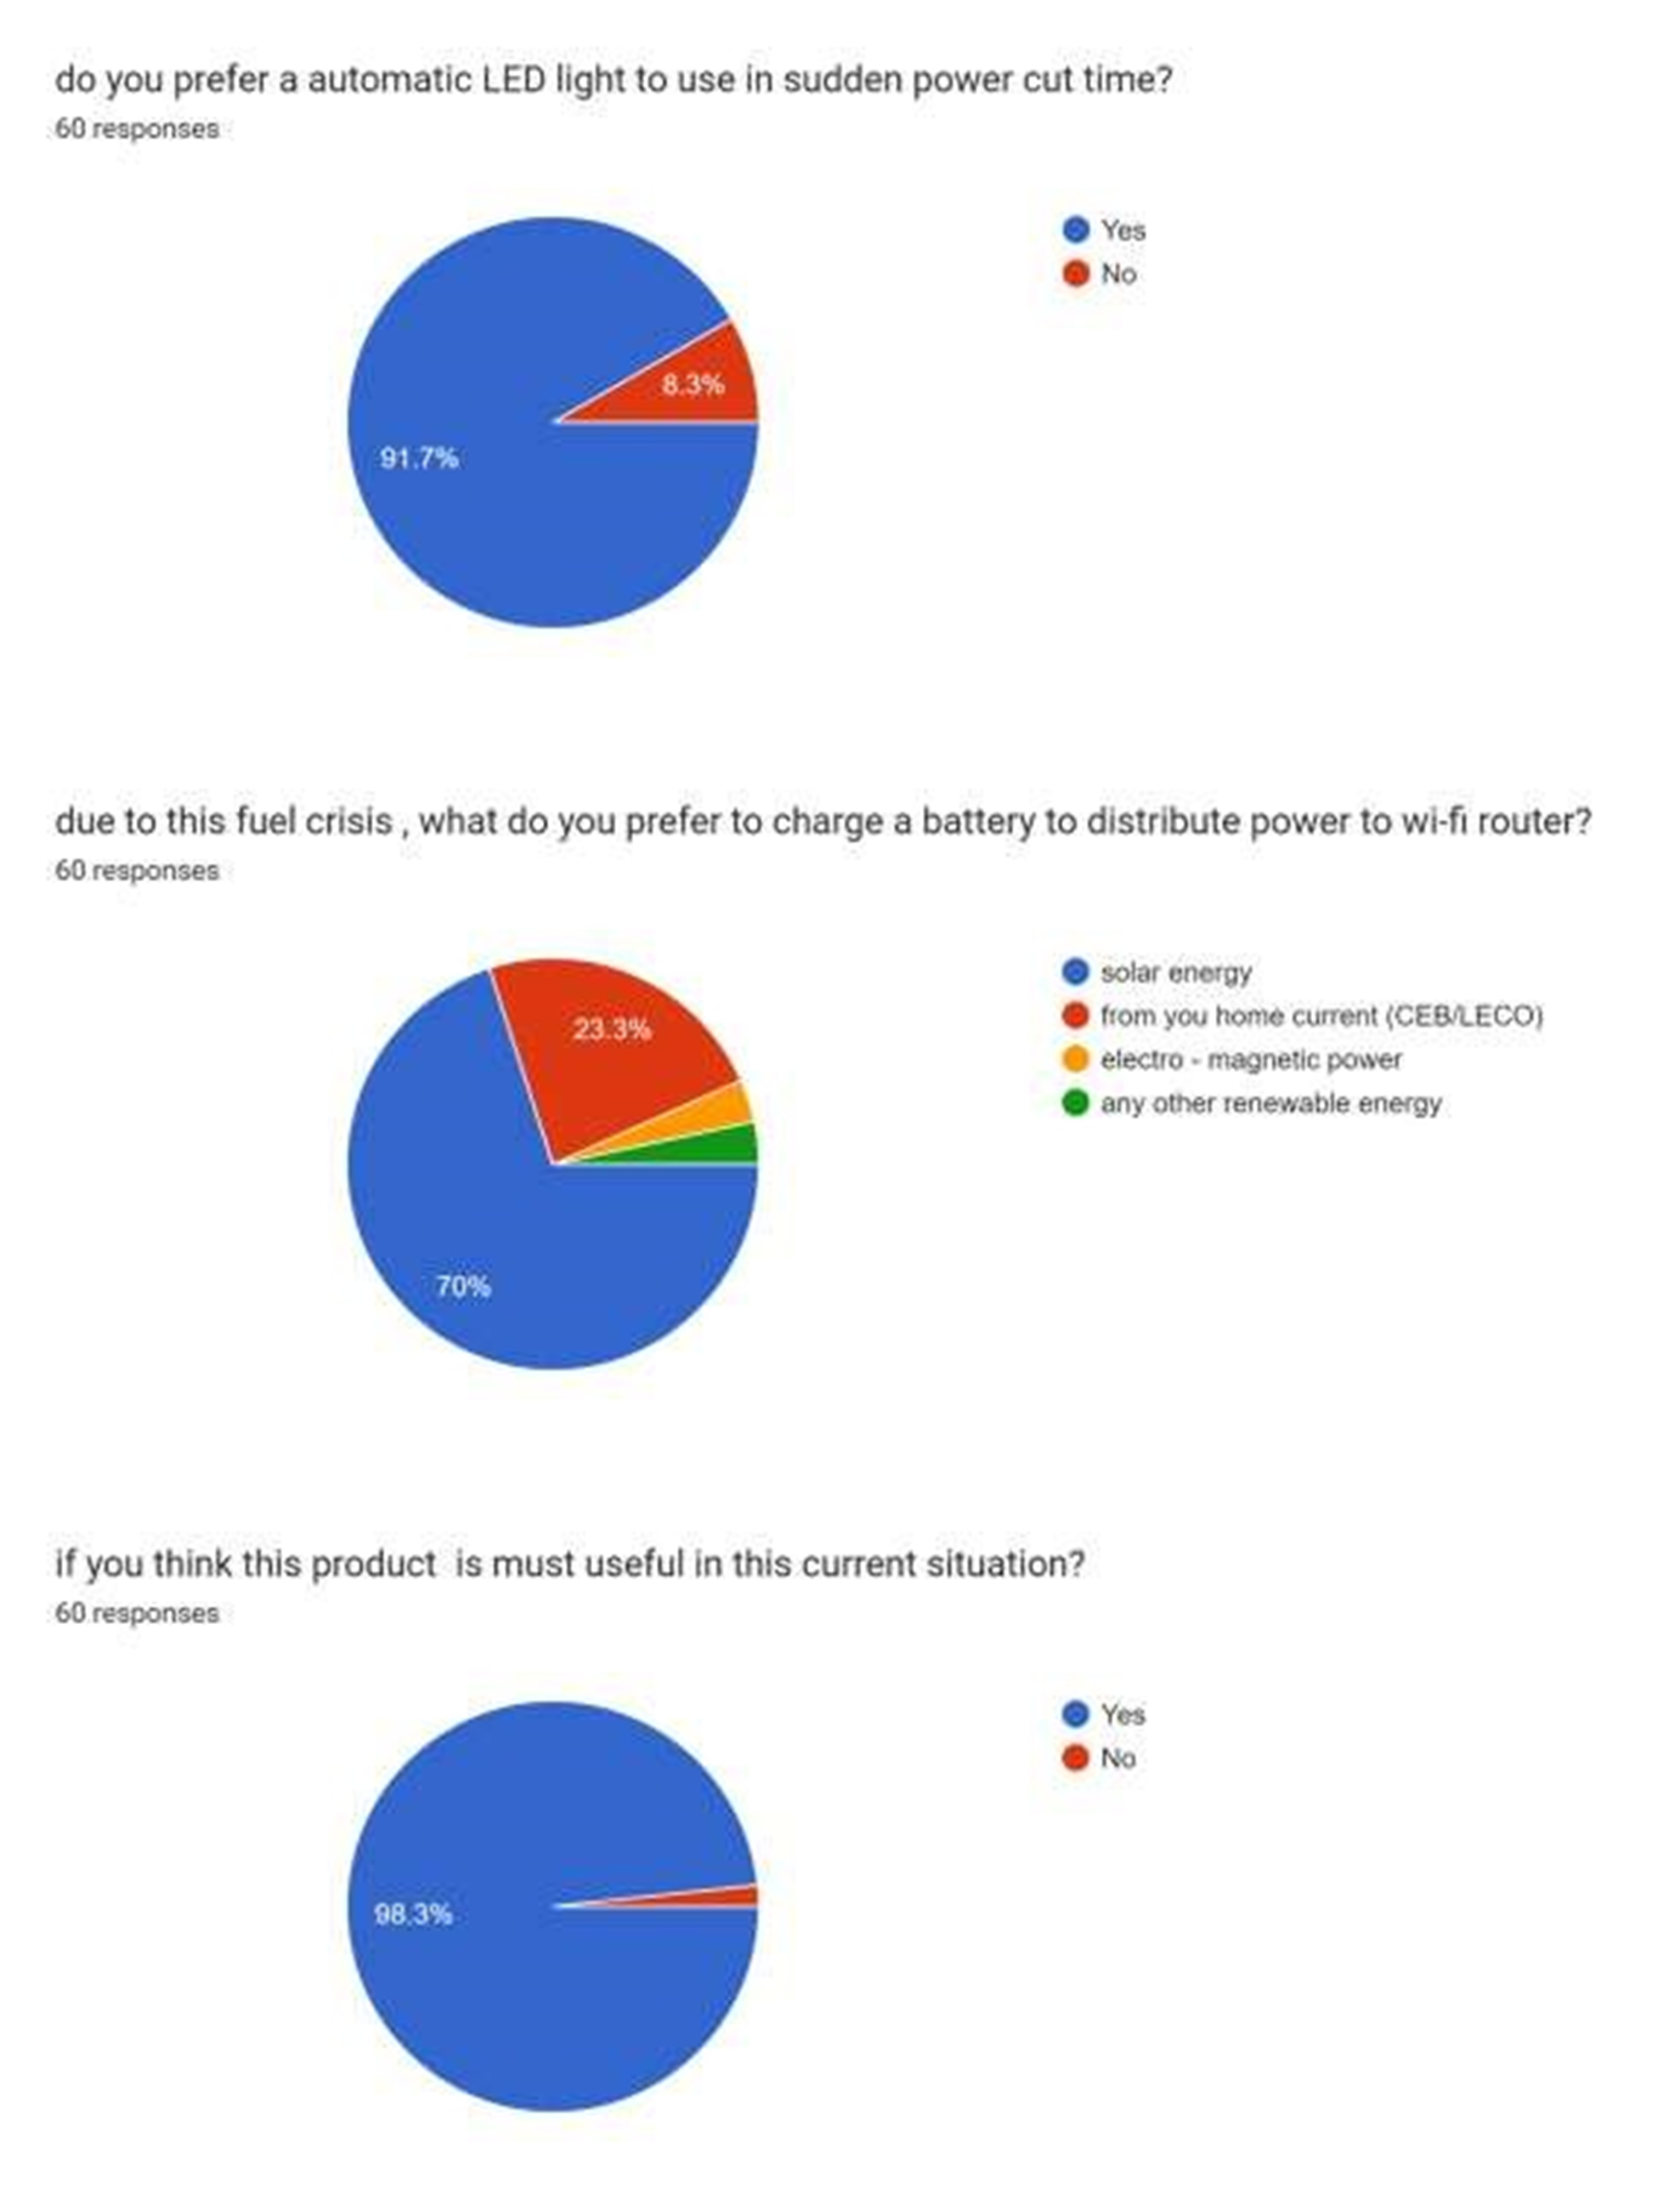
\includegraphics{28.png}
        \label{fig:enter-label}
    \end{figure}

\end{titlepage}

\end{document}



